%  !TeX  root  =  user_guide.tex  

\section{L'extension de géoréférencement}

%The Georeferencer Plugin is a tool for generating world files for rasters.
%It allows you to reference rasters to geographic or projected coordinate 
%systems by creating a new GeoTiff or by adding a world file to the 
%existing image. The basic approach to georeferencing a raster is to locate 
%points on the raster for which you can accurately determine their coordinates. 

L'extension de géoréférencement est un outil permettant de renseigner les coordonnées de rasters en générant les fichiers "world" (fichiers de référence indiquant le système géographique ou de projetion à employer) ou de les transformer dans un nouveau système. La première étape pour le géoréférencement d'une image est de localiser des points sur le raster dont vous pouvez connaissez les coordonnées.

%\minisec{Features}
\minisec{Features}


\begin{table}[h]\index{Georeferencer!tools}
\begin{tabular}{|m{1cm}|m{6cm}|m{1cm}|m{6cm}|}
 \hline \textbf{Icône} & \textbf{Rôle} & \textbf{Icône} & \textbf{Rôle} \\
 \hline 
\includegraphics[width=0.7cm]{mActionAddRasterLayer} & Ouvrir un raster &
   
\includegraphics[width=0.7cm]{mActionStartGeoref} & Commencer le géoréférencement \\
 \hline 
\includegraphics[width=0.7cm]{mActionGDALScript} & Geénérer le script GDAL &
   
\includegraphics[width=0.7cm]{mActionFileOpen} & Charger les points de contrôle \\
 \hline 
\includegraphics[width=0.7cm]{mActionFileSave} & Sauvegarder les points de contrôle &
   
\includegraphics[width=0.7cm]{mActionOptions} & paramètres de transformation \\
 \hline 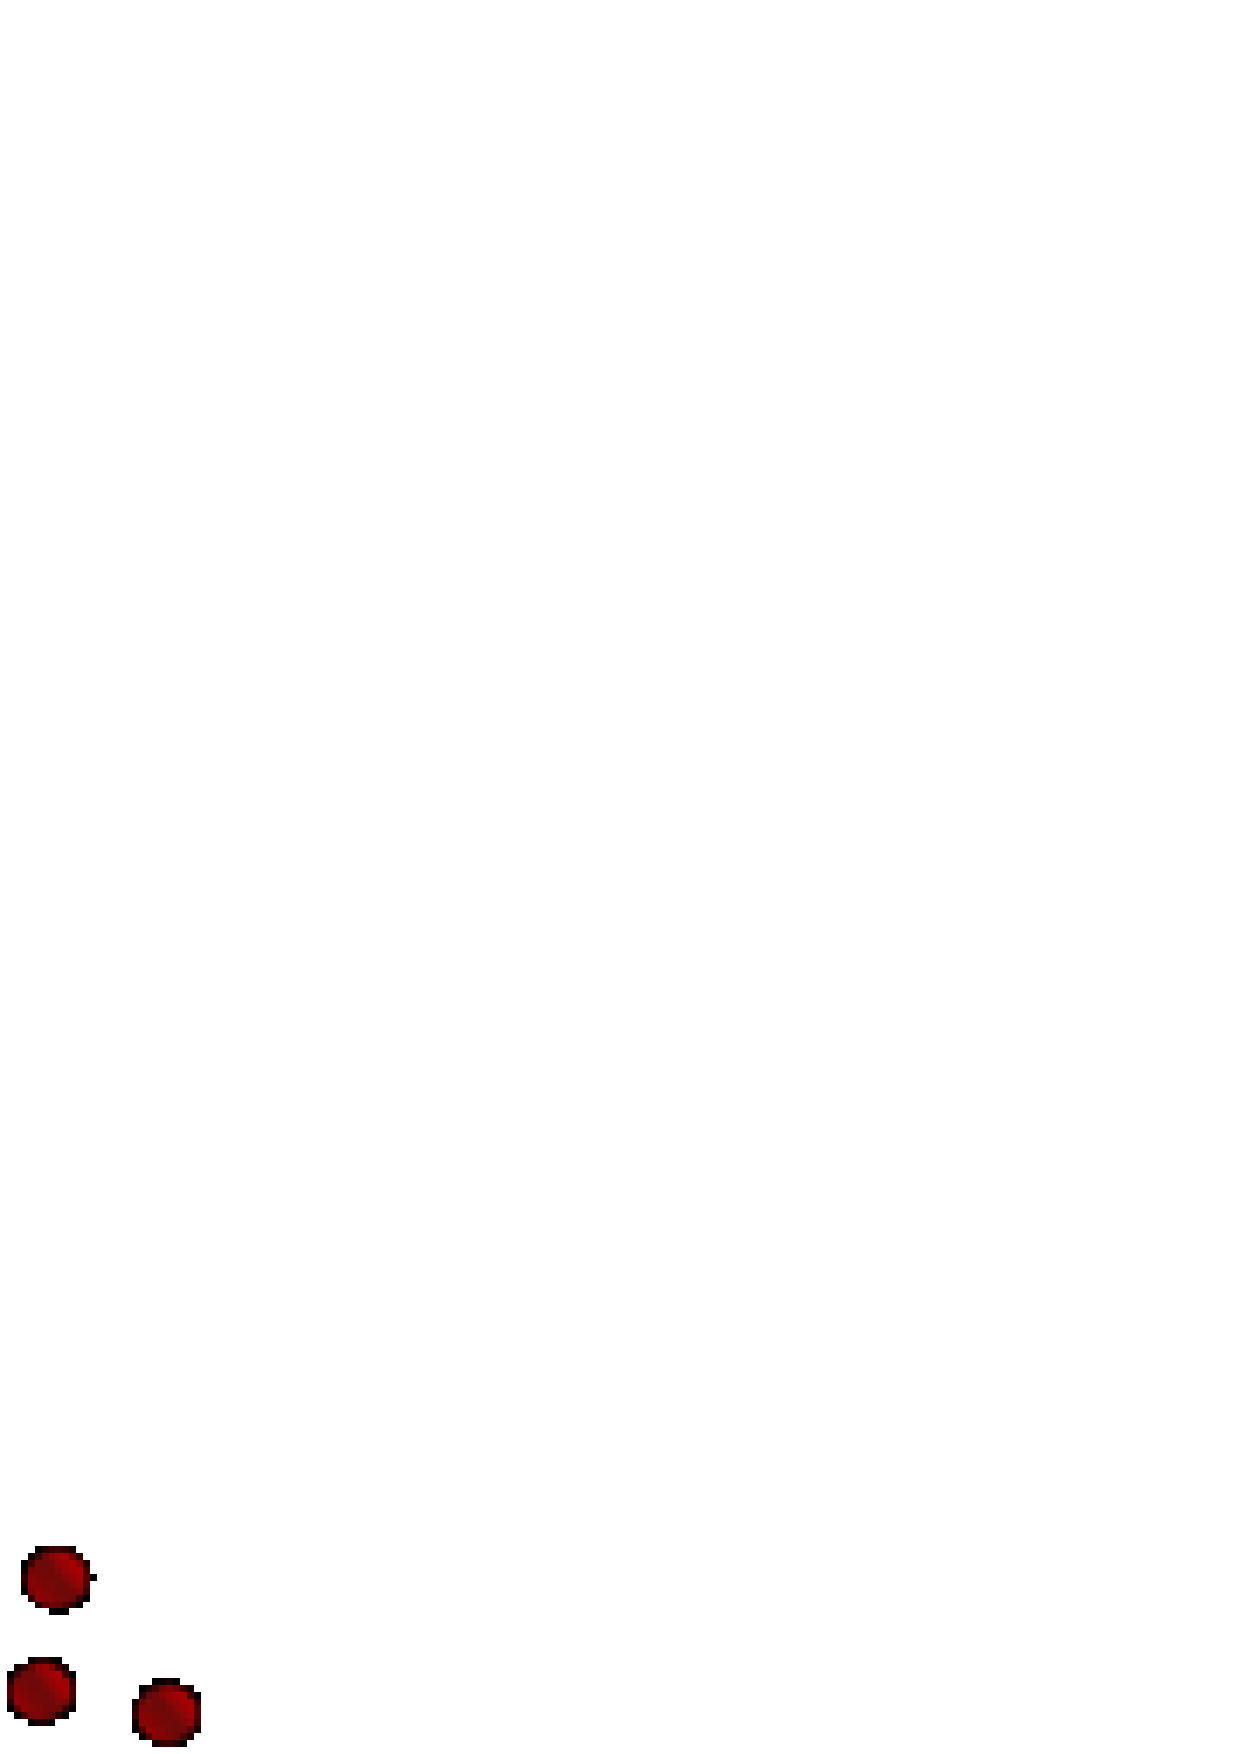
\includegraphics[width=0.7cm]{mActionCapturePoint} & Ajouter Point &
   
\includegraphics[width=0.7cm]{mActionDeleteSelected} & Effacer un point \\
 \hline 
\includegraphics[width=0.7cm]{mActionEditPaste} & Déplacer un point &
   
\includegraphics[width=0.7cm]{mActionPan} & Se déplacer \\
 \hline 
\includegraphics[width=0.7cm]{mActionZoomIn} & Zoom + &
   
\includegraphics[width=0.7cm]{mActionZoomOut} & Zoom - \\
 \hline 
\includegraphics[width=0.7cm]{mActionZoomToLayer} & Zoom sur la couche &
   
\includegraphics[width=0.7cm]{mActionZoomLast} & Zoom précédent \\
 \hline 
\includegraphics[width=0.7cm]{mActionZoomNext} & Zoom suivant &
   
\includegraphics[width=0.7cm]{mActionLinkGeorefToQGis} & Lier le géoréférenceur à QGIS \\
 \hline 
\includegraphics[width=0.7cm]{mActionLinkQGisToGeoref} & Lier QGIS au géoréférenceur &
 &  \\
\hline
\end{tabular}
\caption{Outils de géoréférencement}\label{tab:georeferencer_tools}
\end{table}

%\minisec{Usual procedure}
\minisec{Procédures courantes}

%As X and Y coordinates (DMS (dd mm ss.ss), DD (dd.dd) or projected coordinates 
%(mmmm.mm) which correspond with the selected point on the image, two 
%alternative procedures can be used: 

Avec des coordonnées X et Y (notées en DMS (dd mm ss.ss), DD (dd.dd) ou en coordonnées projetées 
(mmmm.mm) qui correspondent au point sélectionné sur l'image, deux procédures peuvent être suivies :

%\begin{enumerate}
%\item The raster itself, sometimes coordinates are literally `written' on the raster. 
%In this case you can enter the coordinates manually.
%\item Other georeferenced data, this can be either vector or raster data that contain the same objects/features that you have on the raster that you want to georeference. In this case you can enter the coordinates by clicking on the reference dataset loaded in QGIS map canvas.
%\end{enumerate}

\begin{enumerate}
\item par le raster lui-même, quelquefois les coordonnées sont littéralement écrites (p. ex., les graticules). Dans ce cas, vous pouvez les saisir manuellement.
\item par des données déjà géoréférencées, cela peut être des données vecteurs ou rasters qui contient les mêmes objets/entités que le raster que vous désirer géoréférencer. Dans ce cas, il vous faudra renseigner les coordonnées en cliquant les données de référence qui auront été chargées dans la carte principale de QGIS.
\end{enumerate}

%The usual procedure for georeferencing an image involves selecting multiple points on the raster, 
%specifying their coordinates, and choosing a relevant transformation type. Based on the input parameters and data, the plugin will compute the world file parameters. The more coordinates you provide, the better the result will be.

La procédure standard pour lé géoréférencement d'une image implique la sélection de plusieurs points sur le raster, en spécifiant leurs coordonnées et en choisissant la transformation appropriée. En se basant sur les paramètres rentrés et les données, l'extension calculera les paramètres du fichier "world". Plus il y a de coordonnées fournies, meilleur sera le résultat.

%The first step is to start QGIS and load the Georeferencer Plugin (see Section 
%\ref{sec:load_core_plugin}) and click on the \toolbtntwo{georeferencer}{Georeferencer} 
%icon which appears in the QGIS toolbar menu. The Georeferencer Plugin dialog appears as 
%shown in Figure \ref{fig:georefplugin}.

La première étape est de lancer QGIS puis de charger l'extension (voir la section \ref{sec:load_core_plugin}) pour enfin cliquer sur l'icône \toolbtntwo{georeferencer}{Géoreferencer} qui apparaît dans la barre d'outils de QGIS. La fenêtre de géoréférencement se présente sous la forme montrée dans la figure \ref{fig:georefplugin}.
 
%For this example, we are using a topo sheet of South Dakota from SDGS. It can later be visualized 
%together with the data from the GRASS spearfish60 location. You can download the topo sheet here: 
%\url{http://grass.osgeo.org/sampledata/spearfish\_toposheet.tar.gz}

En guise d'exemple, nous allons utiliser un fichier world issu d'une carte topographique du Dakota du Sud publiée par le SDGS.
Elle pourra par la suite être affichée avec les données du secteur GRASS spearfish60. Cette carte topographique peut être téléchargée à l'adresse suivante : \url{http://grass.osgeo.org/sampledata/spearfish\_toposheet.tar.gz}

%\begin{figure}[ht]
%\begin{center}
%  \caption{Georeferencer Plugin Dialog \nixcaption}\label{fig:georefplugin}\smallskip
%  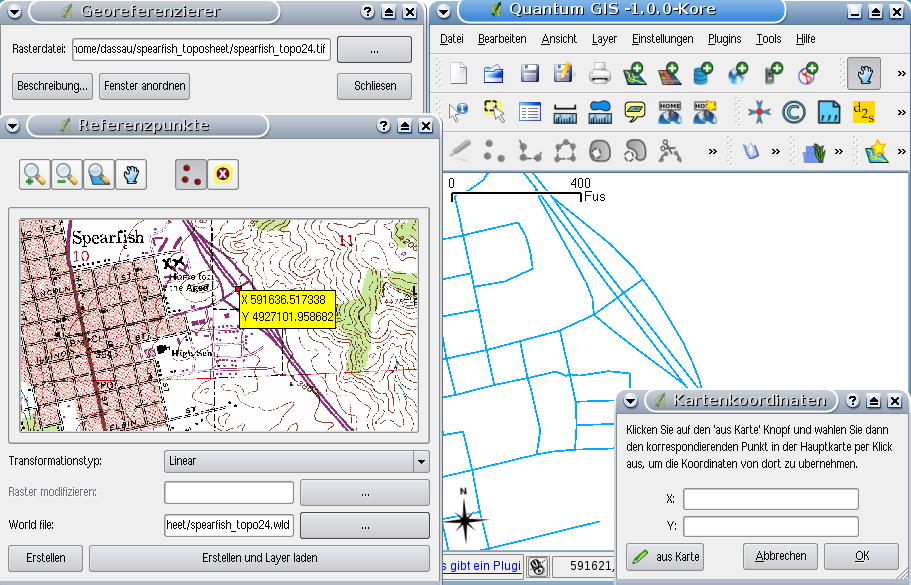
\includegraphics[clip=true, width=12cm]{georefplugin}
%\end{center}
%\end{figure}

\begin{figure}[ht]
\begin{center}
  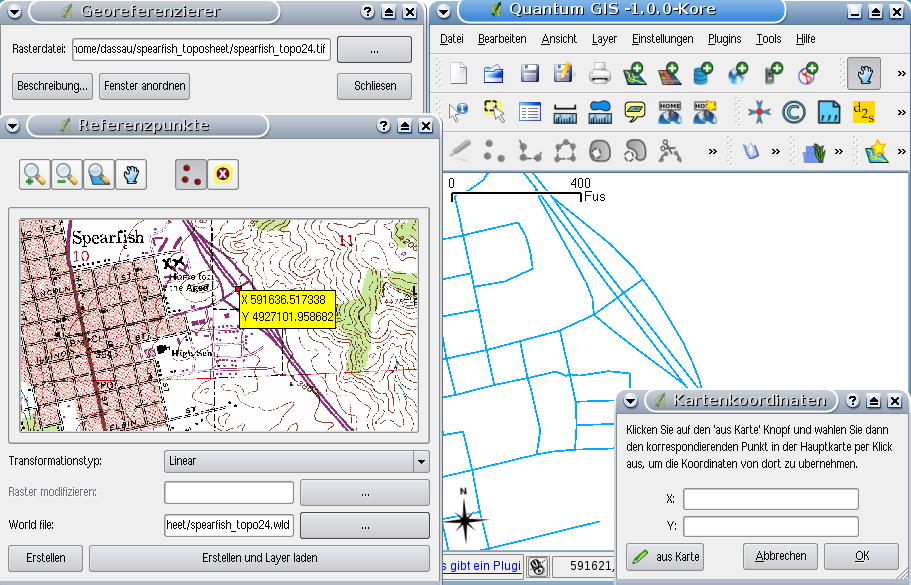
\includegraphics[clip=true, width=10cm]{georefplugin}
  \caption{Fenêtre de l'extension de géoréférencement \nixcaption}\label{fig:georefplugin}
\end{center}
\end{figure}

%\minisec{Entering ground control points (GCPs)}\label{georeferencer_entering}
\minisec{Saisir des points de contrôles (GCP)}\label{georeferencer_entering}

%\begin{enumerate}
%\item To start georeferencing an unreferenced raster, we must load it using the \browsebutton browse button. The raster will show up in the main working area of the dialog. Once the raster is loaded, we can start to enter reference points.
\begin{enumerate}
\item Pour commencer le géoréférencement d'un raster, nous devons le charger via le bouton \browsebutton. Le raster apparaît alors dans la surface principale de travail de la fenêtre. Une fois qu'il est chargé, nous pouvons commencer à entrer des points de coordonnées.

%\item Using the \toolbtntwo{mActionCapturePoint}{Add Point} button, add points to the main working area and enter their coordinates (See Figure \ref{fig:choose_points}). For this procedure you have two options:
\item En utilisant le bouton \toolbtntwo{mActionCapturePoint}{Ajouter des Points}, ajouter par un clic des points dans la surface de travail et saisissez leurs coordonnées (voir figure \ref{fig:choose_points}). Pour ce faire, il y a deux manières de procéder :

\begin{enumerate}
%\item Click on a point in the raster map and enter the X and Y coordinates manually
\item En cliquant en un point de la carte raster et entrant les coordonnées X et Y manuellement
%\item Click on a point in the raster image and choose the button 
%\toolbtntwo{pencil}{from map canvas} to add the X and Y coordinates with the help 
%of a georeferenced map already loaded in the QGIS map canvas.
\item En cliquant en un point de la carte raster puis sur le bouton \button{Depuis le caneva} pour ajouter les coordonnées X et Y à l'aide d'une carte géoréférencée déjà chargée dans le canevas principal de \qg.
%\end{enumerate}
%\item Continue entering points. You should have at least 4 points, and the 
%more coordinates you can provide, the better the result will be. There are 
%additional tools on the plugin dialog to zoom and pan the working area in 
%order to locate a relevant set of GCP points.
\end{enumerate}
\item Continuez de rentrer des points jusqu'à en avoir au moins 4. Des outils additionnels situés dans la partie supérieure de cette fenêtre permettent de zoomer et de se déplacer dans l'espace de travail.
\end{enumerate}

\begin{figure}[ht]
\centering
%  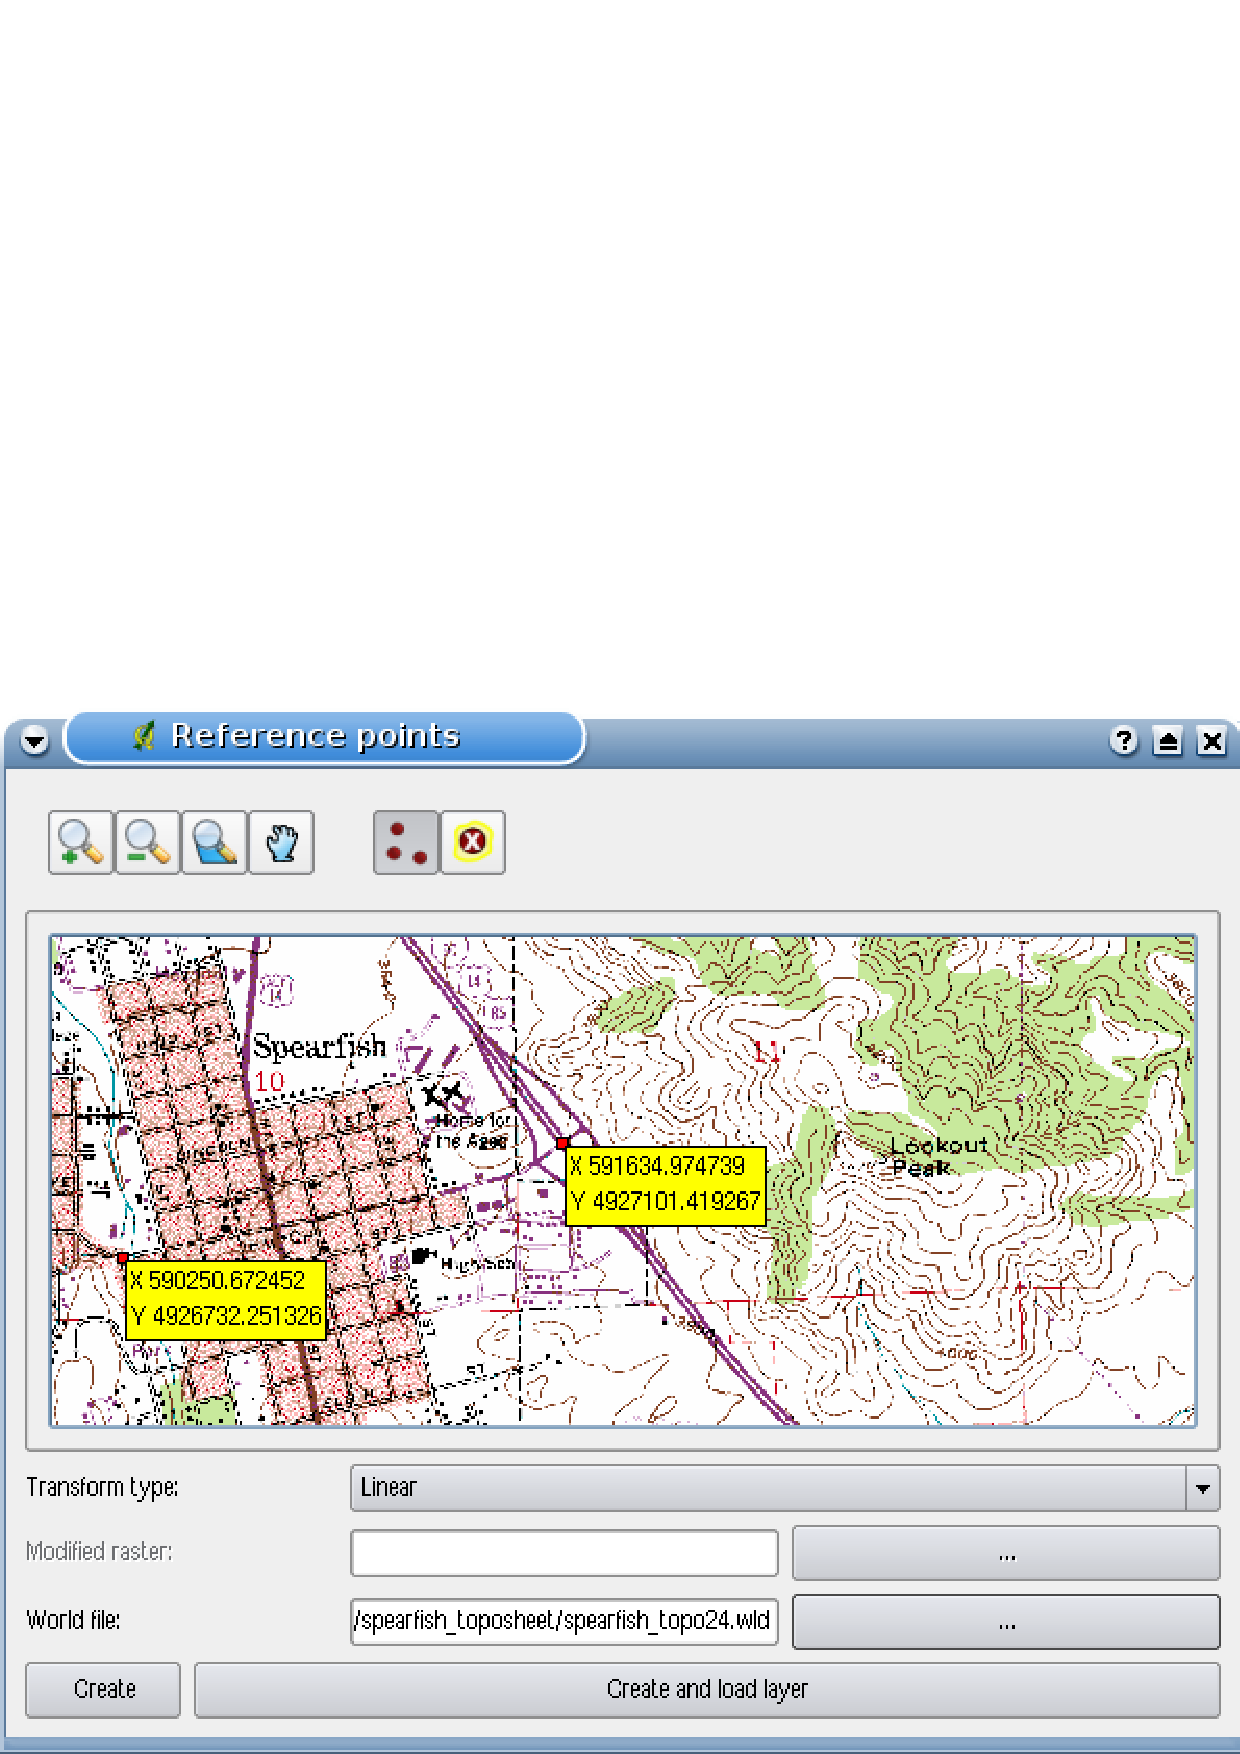
\includegraphics[clip=true,width=9cm]{choose_points}
%  \caption{Add points to the raster image \nixcaption}\label{fig:choose_points}
  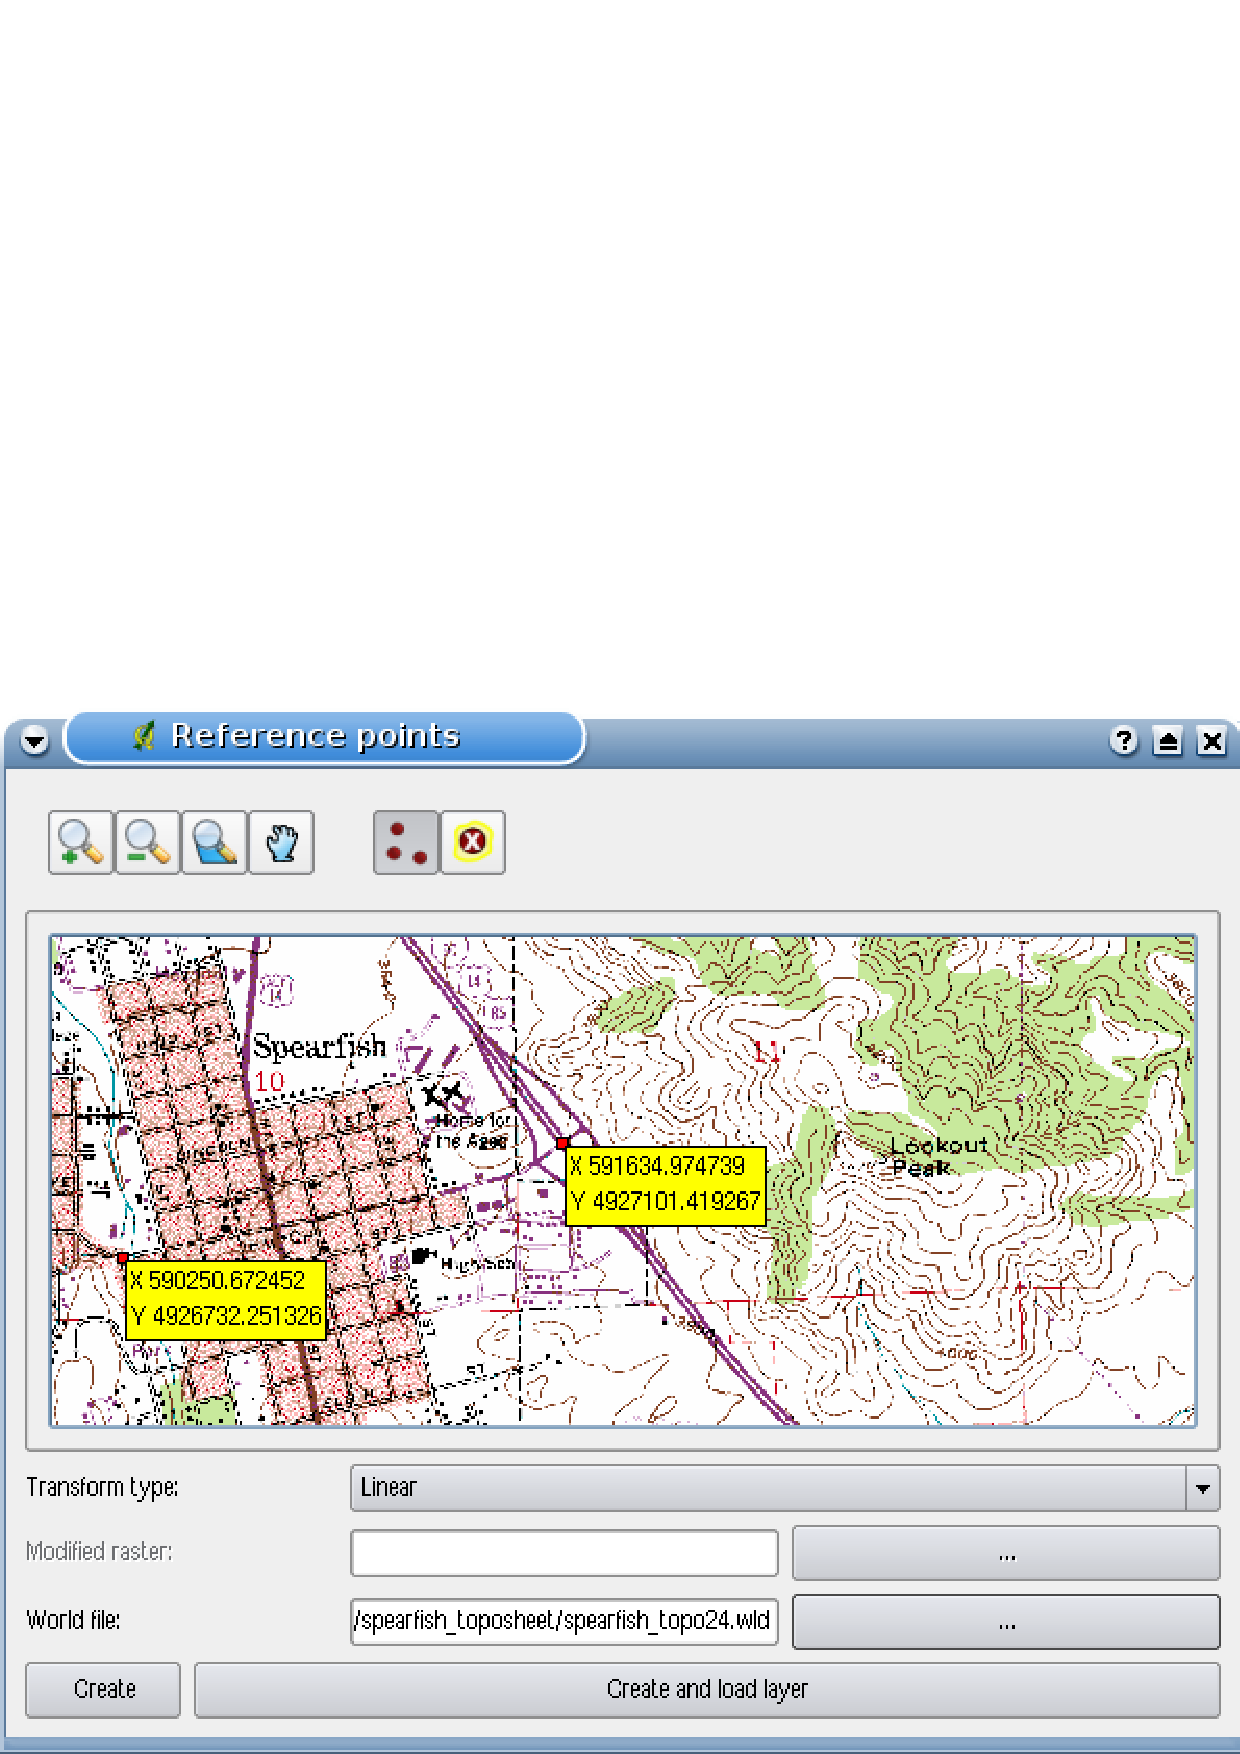
\includegraphics[clip=true,width=9cm]{choose_points}
  \caption{Ajout de points à l'image raster \nixcaption}\label{fig:choose_points}
\end{figure}

%The points that are added to the map will be stored in a separate text file ([filename].points) which is stored together with the raster image. This allows us to reopen the Georeferencer plugin at a later date and add new points or delete existing ones to optimize the result. The points file contains values of the form: mapX, mapY, pixelX, pixelY. You can also \button{Load GCPs} and \button{Save GCPs} to different directories if you like.

The points that are added to the map will be stored in a separate text 
file ([filename].points) usually together with the raster image. 
This allows us to reopen the Georeferencer plugin at a later date and add 
new points or delete existing ones to optimize the result. The points file 
contains values of the form: mapX, mapY, pixelX, pixelY. You can use the 

\includegraphics[width=0.7cm]{mActionFileOpen} 'Load GCP Points' and 

\includegraphics[width=0.7cm]{mActionFileSave} 'Save GCP Points' buttons to 
manage the files.

Les points qui sont ajoutés sur la carte sont enregistrés dans un fichier texte distinct ([nomduichier].points) qui est stocké avec le fichier raster. Il permet de rouvrir l'extension à une date ultérieure et de rajouter de nouveaux points ou d'effacer ceux existants pour améliorer le résultat sans devoir tout refaire. Le fichier de point contient les valeurs suivantes : mapX, mapY, pixelX, pixelY (soit les coordonnées cartographiques et les coordonnées du pixel). Vous pouvez aussi utiliser 
\includegraphics[width=0.7cm]{mActionFileOpen} 'Charger des points de contrôle' et 
\includegraphics[width=0.7cm]{mActionFileSave} 'Sauvegarder des points de contrôle' dans des répertoires différents si vous le désirez.

%\minisec{Choosing the transformation}\label{georeferencer_transformation}
\minisec{Choosing the transformation}\label{georeferencer_transformation}

%After you have added your GCPs to the raster image, you need to select the transformation type for the georeferencing process. Depending on how many ground control point you have captured, you may want to use different transformation algorithms. Choice of transformation algorithm is also dependent on the type and quality of input data and the amount of geometric distortion that you are willing to introduce to final result.

Après avoir ajouté vos points de contrôle, vous devez sélectionner la méthode de transformation qui sera utilisée pour le géoréférencement. Selon le nombre de points que vous avez recueilli, vous devrez utiliser l'algorithme le plus adapté. Le choix de cet algorithme dépend aussi du type et de la qualité des données et de la somme des distorsions géométriques que vous estimerez acceptable pour produire le résultat final.

\begin{figure}[ht]
\centering
%  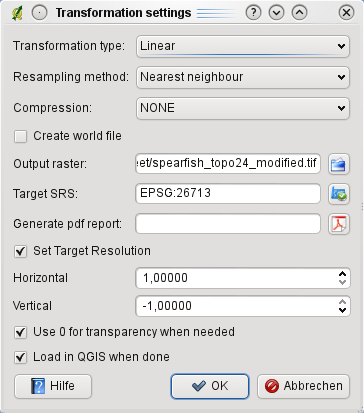
\includegraphics[clip=true,width=8cm]{transformation_settings}
%  \caption{Defining the georeferencer transformation settings \nixcaption}\label{fig:georef_transform}
  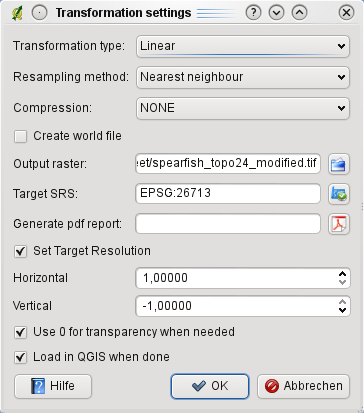
\includegraphics[clip=true,width=8cm]{transformation_settings}
  \caption{Définir les paramètres de transformations \nixcaption}\label{fig:georef_transform}
\end{figure}

%\minisec{Available Transformation algorithms}
\minisec{Algorithmes de transformation disponibles}

%Depending on how many ground control point you have captured, you may want 
%to use different transformation algorithms. Choice of transformation 
%algorithm is also dependent on the type and quality of input data and 
%the amount of geometric distortion that you are willing to introduce 
%to final result.

Selon le nombre de points que vous saisissez, vous aurez à utiliser différents algorithmes de transformation. Le choix d'un algorithme dépend aussi du type et de la qualité de vos sources de données et du niveau de distorsion géométrique que vous êtes prêt à accepter dans le résultat final

%Currently, following algorithms are available: 
Actuellement les algorithmes suivants sont disponibles :

\begin{itemize}[label=--]
%\item The \textbf{Linear algorithm} is used to create a world-file, and is different 
%from the other algorithms, as it does not actually transform the raster. 
%This algorithm likely won't be sufficient if you are dealing with scanned 
%material.
\item L'algorithme \textbf{Linéaire}  is used to create a world-file, and is different  from the other algorithms, as it does not actually transform the raster.  This algorithm likely won't be sufficient if you are dealing with scanned  material.
%\item The \textbf{Helmert transformation} performs simple scaling and rotation 
%transformations. 
\item L'algorithme \textbf{Helmert transformation} performs simple scaling and rotation  transformations.
%\item The \textbf{Polynomial algorithms} 1-3 are among the most widely 
%used algorithms 
%for georeferencing, and each one differs by the degree of distortion 
%introduced to match source and destination ground control points. The 
%most widely used polynomial algorithm is the second order polynomial 
%transformation, which allows some curvature. First order polynomial 
%transformation (affine) preserves colliniarity and allows scaling, 
%translation and rotation only.
\item L'algorithme \textbf{Polynomial algorithms} 1-3 are among the most widely  used algorithms  for georeferencing, and each one differs by the degree of distortion  introduced to match source and destination ground control points. The  most widely used polynomial algorithm is the second order polynomial  transformation, which allows some curvature. First order polynomial  transformation (affine) preserves colliniarity and allows scaling,  translation and rotation only.
%\item The \textbf{Thin plate spline (TPS) algorithm} is a more 
%modern georeferencing  method, which is able to introduce local 
%deformations in the data. This algorithm is useful when very low 
%quality originals are being georeferenced.
\item L'algorithme \textbf{Thin plate spline (TPS) algorithm} is a more  modern georeferencing  method, which is able to introduce local  deformations in the data. This algorithm is useful when very low  quality originals are being georeferenced.
\end{itemize}

\begin{itemize}[label=--]
%\item The Linear algorithm is used to create a world-file, and is different from the other algorithms, as it does not actually transform the raster. This algorithm likely won't be sufficient if you are dealing with scanned material.
\item L'algorithme linéaire est utilisé pour créer un fichier world et diffère des autres dans le fait qu'il ne transforme pas vraiment le raster. Il ne sera sans doute pas satisfaisant si vous avez à faire à des travaux scannés.
%\item The Helmert transformation performs simple scaling and rotation transformations. 
\item La transformation de Helmert réalise une simple mise à l'échelle et une rotation.
%\item The Polynomial algorithms are among the most widely used algorithms for georeferencing, and each one differs by the degree of distortion introduced to match source and destination ground control points. The most widely used polynomial algorithm is the second order polynomial transformation, which allows some curvature. First order polynomial transformation (affine) preserves colliniarity and allows scaling, translation and rotation only.
\item Les algorithmes polynomiaux sont ceux les plus utilisés pour le géoréfrencement, chacun diffère des autres par le degré de distrotion introduit dans la tentative de de se rapprocher de la source originelle et des points de contrôle. Le plus courant est celui de deuxième ordre qui permet de courber l'image. La transformation de premier ordre (affine) préserve l'aspect et permet seulement la mise à l'échelle, le déplacement et la rotation.
%\item The Thin plate spline (TPS) algorithm is a more modern georeferencing method, which is able to introduce local deformations in the data. This algorithm is useful when very low quality originals are being georeferenced.
%\end{itemize}
\item L'algorithme Thin Plate Spline (TPS) est une méthode plus moderne qui est capable d'introduire des déformations sur des secteurs précis de l'image. Il est très pratique quand des sources de faible qualité sont utilisées.
\end{itemize}

%\minisec{Define the Resampling method}
\minisec{Définir la méthode de rééchantillonage}\label{georeferencer_running}

%The type of resampling you choose will likely depending on your input data
%and the ultimate objective of the exercise. If you don't want to change
%statistics of the image, you might want to choose Nearest neighbour,
%whereas a Cubic resampling will likely provide a more smoothed result.
Le type de ré-échantillonnage à effectuer dépendra de votre donnée en entrée et de l'objectif de l'exercice. Si vous ne voulez pas changer les statistiques de l'image, vous devriez sélectionner la méthode du plus proche voisin tandis que le ré-échantillonnage cubique produira un résultat plus lisse.

%It is prossible to choose between five different resampling methods.
Il est possible de choisir entre 5 méthodes de ré-échantillonnage :

\begin{enumerate}
\item Au plus proche voisin
\item Linéaire
\item Cubique
\item Cubic Spline
\item Lanczos
\end{enumerate}

%\minisec{Define the Output raster}
\minisec{Définir le type de raster en sortie}

%There are several options that need to be defined for the georeferenced output 
%raster. 
Plusieurs paramètres doivent être renseignés afin de créer un raster géoréférencé.

\begin{itemize}[label=--]
%\item The checkbox \checkbox{Create world file} is only available, if 
%you decide to use the linear transformation type, because this means that 
%the raster image actually won't be transformed. In this case, the field 
%Output raster is not activated, because only a new world-file will be 
%created.
\item La case \checkbox{Créer une fichier de coordonnées} est uniquement disponible lorsque la méthode de transformation linéaire est choisie, et ce, car votre image ne sera alors pas transformée en sortie. Dans ce cas précis, le champ raster de sortie ne sera pas activé, car seulement le fichier de coordonnées sera créé.
%\item For all other transformation type you have to define an \textbf{Output 
%raster}. As default a new file ([filename]\_modified) will be created in 
%the same folder together with the original raster image. 
\item Pour tous les autres types de transformations, vous pouvez saisir un \textbf{Raster de sortie}. Par défaut, le nouveau fichier s'intitulera ([nomdefichier]\_georef) et sera enregistré dans le même répertoire que le raster originel.
%\item As a next step you have to define the Target SRS} 
%(Spatial Reference System) for the georeferenced raster 
%(see section \ref{label_projections}). 
\item L'étape suivante est la définition du \textbf{SCR cible} pour le raster géoréférencé (lire section \ref{label_projections}). 
%\item If you like, you can also \textbf{generate a pdf report}. It includes 
%information about the used transformation parameters. An image of the 
%residuals and a list with all GCPs and their RMS errors.
\item Si vous le désirez, vous pouvez demander à \textbf{générer un rapport PDF} qui inclut tous les paramètres définis ainsi qu'une image avec tous les résidus et une liste des points de contrôles et leurs erreurs RMS \footnote{L'erreur Root Mean Square (RMS) est une mesure de la différence entre la valeur de départ et la valeur calculée, chaque différence est appelée un résidu.}.
%\item Furthermore you can activate the \checkbox{Set Target Resolution} 
%checkbox and define pixel resolution of the output raster. Default horizontal 
%and vertical resolution is 1,      
\item Vous pouvez cochez la case \checkbox{Définir la résolution de la cible} et préciser la résolution de pixel du raster généré. La résolution horizontale et verticale par défaut est de 1.
%\item The \checkbox{Use 0 for transparency when needed} can be activated, if 
%pixels with the value 0 shall be visualized transparent. In our example 
%toposheet all white areas would be transparent.
\item  Lorsque la case \checkbox{Use 0 for transparency when needed} est cochée, cela indique que la valeur 0 sera transparente lors de la visualisation. Dans notre exemple, toutes les zones blanches seront transparentes.
%\item Finally \checkbox{Load in QGIS when done} loads the output raster 
%automatically into the QGIS map canvas when the transformation is done.
%\end{itemize}
\item Pour finir, la case \checkbox{Charger dans QGIS lorsque terminé} assure le chargement automatique du raster quand la transformation est achevée.
\end{itemize}

%\minisec{Running the transformation}\label{georeferencer_running}
\minisec{Lancer}\label{georeferencer_running}

Lorsque tous les points de contrôle ont été posés et les paramètres de transformation saisis, appuyez sur le bouton 
\includegraphics[width=0.7cm]{mActionStartGeoref} 'Commencer le géoréférencement' pour créer le raster final.
